\chapter{$R(X)$ in complexity one} \label{chap:R(X)}
\chaptermark{The greatest lower bound on Ricci curvature}
Recall, as discussed in the introduction, that one approach to the existence of K\"ahler-Einstein metrics is the study of the continuity path, that is solutions \(\omega_t \in 2 \pi c_1(X) \) to the equation
\[
\Ric(\omega_t) = t\omega_t + (1-t) \omega.
\]
for \(t \in [0,1]\) . By \cite{Yau1977} there is always a solution for \(t = 0\). However, Tian \cite{tian1992stability} showed that for some \(t\) sufficiently close to \(1\) there may not be a solution for certain Fano manifolds. It is natural to ask for the supremum of permissible \(t\), which turns out to be independent of the choice of \(\omega\).
\begin{definition}
Let \((X,\omega)\) be a K\"ahler manifold with \(\omega \in 2 \pi c_1(X)\). Define:
\[
R(X) := \sup ( t \in [0,1]   : \exists \ \omega_t \in 2 \pi c_1(X)  \ \Ric( \omega_t) = t \omega_t + (1-t) \omega ).
\]
\end{definition}
This invariant was first discussed, although not explicitly defined, by Tian in \cite{Tian87}. It was first explicitely defined by Rubenstein in \cite{rubinstein2008} and was further studied by Szekelyhidi in \cite{szekelyhidi2011}. It is sometimes referred to as the greatest lower bound on Ricci curvature.

In \cite{rubinstein2008} Rubenstein showed relation between \(R(X)\) and Tian's alpha invariant \(\alpha(X)\), and in \cite{rubinstein2009} conjectured that \(R(X)\) characterizes the \(K\)-semistability of \(X\). This conjecture was later verified by Li in \cite{li2017}.

In \cite{li2011} Li  determined a simple formula for \(R(X_\Delta)\), where \(X_\Delta\) is the polarized toric Fano manifold determined by a reflexive lattice polytope \(\Delta\). This result was later recovered in \cite{datar2016kahler}, by Datar and Sz\'ekelyhidi, using notions of \(G\)-equivariant \(K\)-stability. Previously \(R(X)\) has been calculated for group compactifications by Delcroix \cite{delcroix2017} and for homogeneous toric bundles by Yao \cite{yao2017}. Let us briefly recall the toric formula.
\begin{theorem}[Li]
Suppose \(X\) is a smooth Fano toric variety. Let \(P\) be the corresponding Fano polytope. If \(\bc(P) = 0\) then \(X\) is K\"ahler-Einstein and \(R(X) = 1\). Otherwise let \(q\) be the intersection of the ray generated by \(-\bc(P)\) with the boundary \(\partial P\). We then have:
\[
R(X) = \frac{|q|}{|q-\bc(P)|}.
\]
\end{theorem}

\begin{example}
Consider the toric variety \(X = \Bl_z \PP^1 \times \PP^1\) from Example~\ref{}. It is then easy to calculate \(R(X)\) from the polytope \(P\) given in Example~\ref{}. We have \(\bc(P) = (-2/21,-2/21)\) and \(q = (1/2,1/2)\) so \(R(X) = 21/25\).
\begin{figure}[h]
\centering
  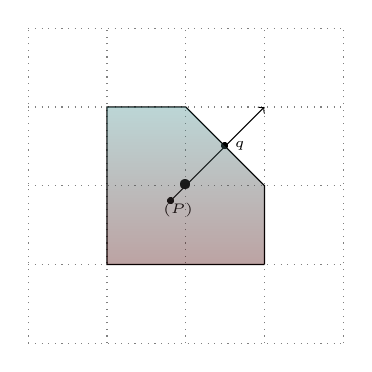
\begin{tikzpicture}[scale=1]
   	 \draw[dotted,step=1,gray,] (-2,-2) grid (2,2);
   	 \draw[] (1,-1) -- (1,0) -- (0,1) -- (-1,1) -- (-1,-1) -- (1,-1);
   	 \draw (0,0) node {\textbullet};
   	 \draw (-2/21,-2/21) node[below] {\tiny{$\bc(P)$}};
  	 \draw (-4/21,-4/21) node {\tiny{\textbullet}};
   	 \draw (1/2,1/2) node {\tiny{\textbullet}};
  	 \draw (1/2,1/2) node[right] {\tiny{$q$}};
   	 \draw [->] (-4/21,-4/21) -- (1,1);
   	 \fill[bottom color=red!50!black, top color=cyan!50, opacity=0.2]
    (1,-1) -- (1,0) -- (0,1) -- (-1,1) -- (-1,-1) -- (1,-1);  	 
	\end{tikzpicture}
	\caption{$R(X)$ calculation for a toric $X$}
\end{figure}
\end{example}

Using similar methods to \cite{datar2016kahler} we obtain an effective formula for manifolds with a torus action of complexity one, in terms its divisorial polytope. Let \(\Phi: \Box \to \div \PP^1\) be the Fano divisorial polytope corresponding to a smooth Fano complexity one \(T\)-variety \(X\). Let \(\{\Delta_i\}_{i=1,\dots,r}\) be finite set of degeneration polytopes corresponding to central fibres of the non-product test configurations of \(X\), as described in \ref{subsec:IS}.

To state our result we must introduce a little more notation. Suppose we have \(\bc(\Delta_i) \neq 0\) for some i. Let \(F_i\) be  the face of \(\Delta_i\) in which \(q_i\) lies, and let \(S\) be the set of indices \(i\) for which \(\bc(\Delta_i) \neq 0\) and all outer normals to \(F_i\) lie in \(H\).


Recall the definition of the Duistermatt Heckman measure \(\nu\), and associated weighted barycenter of \(\Box\) given in \ref{subsec:IS}. Suppose \(\bc_\nu(\Box) \neq 0\). Let \(q\) be the intersection of the ray generated by \(-\bc_\nu(\Box)\) with \(\partial \Box\). Consider the halfspace \(H := N_\RR \times \RR^+ \subset N'_\RR\). Let \(q_i\) be the point of intersection of \(\partial \Delta_i\) with the ray generated by \(-\bc(\Delta_i)\).

Note, by the equation for the Donaldson Futaki invariants \ref{eq:futaki-character} and Theorem~\ref{thm:DS}, we know that \(R(X) = 1\) iff \(\bc_\nu(\Box) = 0\) and \(S = \emptyset\). We may now state our result:

\begin{theorem}[{\cite[Theorem 1.1]{cable2019greatest}}] \label{thm:R(X)} Let \(X\) be a complexity one Fano \(T\)-variety as above. If \(\bc_\nu(\Box) = 0\) and \(S = \emptyset\) then \(R(X) = 1\). Otherwise:
\[
R(X) = \min \  \left\lbrace \frac{|q|}{|q-\bc_\nu(\Box)|}  \ \right\rbrace \cup \ \left\lbrace \frac{|q_i|}{|q_i - \bc(\Delta_i)|} \right\rbrace_{i \in S} .
\]
\end{theorem}
\begin{example}
Consider the \((\CC^*)^2\)-threefold 2.30 from example \ref{}. There are \(3\) normal toric degenerations, given by the polytopes \(\Delta_1,\dots,\Delta_3\). It can be checked in this case that \(S = \emptyset\), as for each \(i\) there is an outer normal \(n_i \not\in H\) to the face \(F_i\). See Figure 1 (a) for an example.
\begin{figure}[H]
\centering
\begin{subfigure}[t]{0.4\textwidth}
\begin{tikzpicture}[%
    tdplot_main_coords,
    scale=0.6,
    >=stealth
  ]
  \draw[->, ultra thick, opacity = 1] (0, 18/46, -57/184)  -- (0, 0.6, -1.1) node[right]{$n_1$} ;
    \draw[fill=white,opacity=1] (0,-3,1) -- (-3,0,1) -- (3,0,-2) -- cycle;
    \draw[fill=white,opacity=0] (3,0,-2) -- (-3,0,1) -- (-2,1,1) -- (2,1,-1) -- cycle;
    \filldraw[ultra thick, opacity = 1] (0, -6/23, 19/92) circle (1pt) node[above]{$\bc(\Delta_1)$}  -- (0,0,0) circle (1pt) node[below]{O} -- (0, 18/46, -57/184) circle (1pt) node[right]{$q_1$}	 ;
    \draw[fill=white,opacity=0.5] (0,-3,1) -- (-3,0,1) -- (-2,1,1) -- (0,1,1) -- cycle;
    \draw[fill=white,opacity=0.5] (0,-3,1) -- (0,1,1) -- (2,1,-1) -- (3,0,-2) -- cycle;
    \draw[fill=white,opacity=0.5] (0,1,1) -- (-2,1,1) -- (2,1,-1) -- cycle;
     \draw[->,dotted] (0,0,0) -- (0,0,2);
    \draw[->,dotted] (0,0,0) -- (3,0,0);
    \draw[->,dotted] (0,0,0) -- (0,2,0);
\end{tikzpicture}
\caption{The toric degeneration \(\Delta_1\)}
\end{subfigure}
\qquad \qquad \qquad
\begin{subfigure}[t]{0.2\textwidth}
\begin{tikzpicture}[scale = 0.6]
\draw (-2,1) -- (-3,0) -- (-3,0) -- (0,-3) -- (3,0) -- (2,1) -- cycle ;
\filldraw[ultra thick, opacity = 1] (0,-6/23) circle (1pt) node[below]{$\bc_\nu(\Box)$}  -- (0,0) circle (1pt) node[right]{O} -- (0, 1) circle (1pt) node[above]{q}	 ; 
    \draw[dotted] (-4,0) -- (4,0);
    \draw[dotted] (0,-4) -- (0,2);
\end{tikzpicture}
\caption{The moment polytope \(\Box\).}
\end{subfigure}
\caption{Determining \(R(X)\) for threefold 2.30.}
\end{figure}
Therefore \(R(X)\) is given by the first term in the minimum. We calculate \(\bc_\nu(\Box)= (0,-6/23)\) and \(q = (0,1)\). Then:
\[
R(X) = \frac{1}{1+ 6/23} = \frac{23}{29}.
\]
\end{example}
\begin{corollary}[{\cite[Corollary 1.2]{cable2019greatest}}] \label{cor:R(X)}
In the table below we calculate \(R(X)\) for \(X\) a Fano threefold  admitting a \(2\)-torus action appearing in the list of Mori and Mukai \cite{mori1981classification}. We include only those where \(R(X) <1\). Note all admit a K\"ahler-Ricci soliton by Theorem~\ref{thm:sol}.
\end{corollary}
\begin{table}[H] \centering
\captionsetup{width=.95\linewidth}
\caption{Calculations for complexity \(1\) threefolds appearing in the list of Mori and Mukai for which \(R(X) <1\)}
\begin{tabular}{l l}
\hline
X & R(X) \\
\hline
2.30 & \(23/29\) \\
2.31 & \(23/27\) \\
3.18 & \(48/55\) \\
3.21 & \(76/97\) \\
3.22 & \(40/49\) \\
3.23 & \(168/221\) \\
3.24 & \(21/25\) \\
4.5* & \(64/69\) \\
4.8 & \(76/89\) \\
\hline
\end{tabular}
\label{table:name}
\end{table}
\section{A short digression into convex geometry}
Let \(X\) be a \(T\)-variety of complexity one associated to a divisorial polytope \(\Psi: \Box \to \div(\PP^1)\), see Section~\ref{prelim:Tvar}.
It follows from Theorem~\ref{thm:sze} that:
\begin{align*}
R(X) = \inf_{(\X,\L)}( \sup(t | \DF_t(\X,\L) \ge 0) ),
\end{align*}
where \((\X,\L)\) varies over all special test configurations for \((X,L)\). We have an explicit description of special test configurations and their Donaldson Futaki invariants, see section~\ref{}. We will calculate \(R(X)\) by considering first the product configurations and then the non-product ones. To calculate the values \(\sup(t | \DF_t(\X,\L) \ge 0)\) for a given configuration we need to first consider some elementary convex geometry.

Let \(V\) be a real vector space and \(P \subset V\) be a convex polytope containing the origin, with \(\dim P = \dim V\). Fix some point \(b \in \text{int}(P)\). Let \(q \in \partial P\) be the intersection of \(\partial P\) with the ray \(\tau = \RR^+ (-b)\). Suppose \(n \in V^\vee\) is an outer normal to a face containing \(q\). For \(a \in \partial P\) write \(\mathcal{N}(a) = \{w\in V^\vee \ | \langle a,w \rangle = \max_{x \in P} \langle x,c \rangle \}\). For \(w \in \mathcal{N}(a) \) let \(\Pi(a,w)\) be the affine hyperplane tangent to \(P\) at \(a\) with normal \(w\). For \(w \in \inte(\tau^\vee) \) there is a well-defined point of intersection of \(\Pi(a,w)\) and \(\tau\) which we denote \(p_w\). See Figure~\ref{schematic} for a schematic.
\begin{figure}[h] \centering
\diagram1
\caption{An Example in \(V \cong \RR^2\)}
\label{schematic}
\end{figure}
\begin{lemma} \label{R(X):Lemma3.1}
Fix \(w \in \inte(\tau^\vee) \backslash (\RR^+ n)\). For \(s \in [0,1]\) set \(w(s) := sn + (1-s)w\). As \(n \in \tau^\vee \) we may consider \(p(s) := p_{w(s)}\). For \(0 \le s' < s \le 1\) we then have:
\[
\frac{|p(s)|}{|p(s)-b|} < \frac{|p(s')|}{|p(s')-b|}.
\]
\end{lemma}
\begin{proof}
Without loss of generality we may assume \(s' = 0\). For \(s \in [0,1]\) the points \(p(s), q,b\) are collinear, so \(|p(s)|= |p(s)-q|+|q|\) and \(|p(s)-b| =|p(s)-q| +|q| + |b| \). Therefore:
\[
\frac{|p(s)|}{|p(s) - b|} = \frac{|p(s)-q|+|q|}{|p(s)-q| +|q| + |b|}.
\]
Hence it is enough for \(|p(s)-q| < |p(0)-q|\) whenever \(s >0\). Since \(q \neq 0\) is fixed this is equivalent to:
\[
\frac{|p(s) - q|}{|q|} < \frac{|p(0) - q|}{|q|}.
\]
For each \(s \in [0,1]\) choose \(a(s) \in \partial P\) such that \(w(s) \in \mathcal{N}(a(s))\). Write \(a = a(0)\) for convenience. We then have:
\[
\frac{|p(s)-q|}{|q|} = \frac{\langle a(s)-q, w \rangle }{\langle q,w \rangle}.
\]
Note \(n \in \mathcal{N}(q)\). Now \(\langle a(s)-q,n \rangle \le 0\)  and \( \langle a(s) - q,w \rangle \le \langle a - q,w \rangle\). Clearly we have \(\langle q , n \rangle > 0\). Then:
\begin{align*}
\frac{\langle a(s) - q, w(s) \rangle }{\langle q, w(s) \rangle} &= \frac{s\langle a(s)-q, n \rangle + (1-s)\langle a(s)-q,w \rangle}{s \langle q , n \rangle + (1-s) \langle q, w \rangle} \\ &\le \frac{(1-s)\langle a-q, w \rangle }{s \langle q , n \rangle + (1-s) \langle q, w \rangle} \\ &< \frac{\langle a-q, w \rangle }{\langle q,w \rangle}.
\end{align*}
\end{proof}
\begin{corollary}
Let \(V,P,b,q,\tau,n\) be as in the introduction to this section. Fix some open halfspace \(H \subset V^\vee\) given by \(u \ge 0\) for some \(u \in V \backslash \{0\}\). This defines a projection map \(\pi: V \to V/\langle u \rangle.\) Consider the function \(F_b: V^\vee \times  [0,1] \to \RR\) given by:
\[
F_b(w,t) := t \langle b,w \rangle+ (1-t) \max_{x \in P} \langle x, w \rangle
\]
For any \(W \subseteq V^\vee\) containing \(n\) we have:
\begin{equation} \label{R(X):1}
\sup (t \in [0,1] \ | \ \forall_{w \in W} \  F_b(t,w) \ge 0) = \frac{|q|}{|q-b|}.
\end{equation}
If for some choice of \(n\) we have \(n \not\in H\) then:
\begin{equation} \label{R(X):2}
\sup (t \in [0,1] \ | \ \forall_{w \in H} \  F_b(t,w) \ge 0) = \frac{|\tilde{q}|}{|\tilde{q} - \pi(b)|},
\end{equation}
where \(\tilde{q}\) is the intersection of the ray \(\pi(\tau)\) with the boundary of \(\pi(P)\).
\end{corollary}
\begin{proof}
Note that:
\[
\sup (t \in [0,1] \ | \ \forall_{w \in W} \  F_b(t,w) \ge 0) = \inf_{w \in W} \sup (t \in [0,1] \ | \  F_b(t,w) \ge 0).
\]
Moreover \(\sup (t \in [0,1] \ | \  F_b(t,w) \ge 0) = 1 > F_b(t,n)\) for \(\langle b,w \rangle \ge 0\), so without loss of generality we may assume \(W \subseteq \inte(\tau^\vee)\). For \(w \in W\) then:
\begin{align*}
\sup (t \in [0,1] \ | \  F_b(t,w) \ge 0) &= \frac{\max_{x \in P} \langle x, w \rangle}{ \max_{x \in P} \langle x, w \rangle - \langle b, w \rangle } \\ &= \frac{ \langle a,w \rangle}{\langle a ,w \rangle - \langle b,w \rangle} \\ &= \frac{ \langle p_w,w \rangle}{\langle p_w ,w \rangle - \langle b,w \rangle} = \frac{|p_w|}{|p_w-b|}.
\end{align*}
Hence:
\[
\sup (t \in [0,1] \ | \ \forall_{w \in W} \  F_b(t,w) \ge 0) = \inf_{w \in W} \frac{|p_w|}{|p_w-b|}.
\]
Now for \(w \in W\) consider the continuity path \(w(s) = sn + (1-s)w\). By Lemma \ref{R(X):Lemma3.1} if \(n \in W\) then the above infimum is attained when \(s=1\) and we obtain (\ref{R(X):1}). Otherwise the infimum is attained at some \(w \in \partial W\). For (\ref{R(X):2}) restricting \(F_b\) to \(\partial H \times [0,1]\) gives:
\begin{align*}
F_b(w,t) =  t \langle \pi(b) ,w \rangle+ (1-t) \max_{x \in \pi(P)} \langle x, w \rangle.
\end{align*}
Applying (\ref{R(X):1}) to the polytope \(\pi(P)\) in the vector space \(\partial H\) we obtain (\ref{R(X):2}).
\end{proof}
\section{Proof of Theorem 4}
\subsection{Product Configurations}
Recall the formula for the Donaldson-Futaki invariant of a product configuration \(\X \cong X \times \A^1\) given in section~\ref{}. In particular the restriction of \(\lambda\) to \(\X_0\) is given by a choice of \(w \in N\), and we have:
\begin{align*}
\DF_t(\X,\L)(w) &=   \DF(\X,\L)(w) + \frac{(1-t)}{V} \int_{X} (\max \theta_w - \theta_w) \omega^n \\ &= \langle  \bc(\Psi), w \rangle + \frac{(1-t)}{\vol \Psi} \int_\Box \max_{x \in \Box} \langle x,w \rangle  - \langle \cdot, w \rangle d \eta \\
&= t \langle  \bc(\Psi), w \rangle + (1-t)\max_{x \in \Box} \langle x,w \rangle.
\end{align*}
Let \(q \in N_\RR\) be the point of intersection of the ray generated by \(-\bc(\Psi)\) with \(\partial \Box\). Applying (\ref{R(X):1}), we obtain:
\[
\sup(t | \DF_t(\X,\L) \ge 0) = \frac{|q|}{|q-\bc_\nu(\Box)|}.
\]
\subsection{Non-Product Configurations}
Recall the description of special non-product test configurations of \(X\) from \ref{subsec:IS}. In particular each such configuration \((\X,\L)\) has toric central fiber \(X_{\Delta_i}\) \(\Delta_i\) where \(\Delta_i\) is one of the degeneration polytopes of \ref{}. The restriction of \(\lambda\) to \(\X_0\) may be assumed to be given by some \(v' = (-v,1) \in N_\QQ \). Recall the formula for the twisted Donaldson-Futaki from \ref{}:
\[
\DF_t( \X, \L )  = t \langle \bc(\Delta_y), v' \rangle + (1-t) \max_{x \in \Delta_y} \langle x, v' \rangle.
\]
Set \(H := N_\RR \times \RR^+\).
\begin{proposition}
For any non-product configuration \((\X,\L)\) with special fiber one of the \(\Delta_i\) above, let \(\sigma_i\) be the cone of outer normals to \(\Delta_i\) at the unique point of intersection of \(\partial \Delta_i\) with the ray generated by \(-\bc(\Delta_i)\). Denote this point of intersection by \(q_i\). Then:
\[
\sup(t | \DF_t(\X,\L) \ge 0) =\begin{cases} 
     \frac{|q_i|}{|q_i - \bc(\Delta_i)|} & \sigma_i \cap H \neq \emptyset ;\\ \\
      \frac{|q|}{|q-\bc_\nu(\Box)|} & \sigma_i \cap H = \emptyset.
   \end{cases}
\]
\end{proposition}
\begin{proof}
Extend \(\DF_t(\X,\L)\) linearly to the whole of \(N_\RR \times \RR\). In the case \(\sigma_i \cap H \neq \emptyset\) we may apply (1) from Corollary 2 with \(P = \Delta_i\) and \(b = \bc(\Delta_i)\). Otherwise we may apply (\ref{R(X):2}), noting that \(\pi(\Delta_i) = \Box\) and \(\pi(\bc(\Delta_i)) = \bc_\nu( \Box)\).
\end{proof}
\begin{proof}[Proof of Theorem~\ref{thm:R(X)}]
With Remark 2 in mind, observe that a special test configuration must either be product or non-product. Any non-product configurations \(\Delta_i\) with \(\sigma_i \cap H \neq \emptyset\) have their contribution to the infimum already accounted for and we may exclude them. The result follows.
\end{proof}
\begin{proof}[of Corollary~\ref{cor:R(X)}]
We calculate unit outer normals \(n_i \) of \(F_i\) for every degeneration polytope of each threefold in this list, see \ref{appendix1}. In each case we observe \(n_i \notin H\). The divisorial polytopes and Duistermaat-Heckman measures were originally given in \cite{suss2013fano}, and may be also be found in Appendix~\ref{appendix1}. We may then calculate \(R(X)\) using just the base polytope \(\Box\) and its Duistermaat-Heckman barycenter.
\end{proof}